% \textbf{Title: Poles and Zeroes 2}

Consider this pole-zero map.

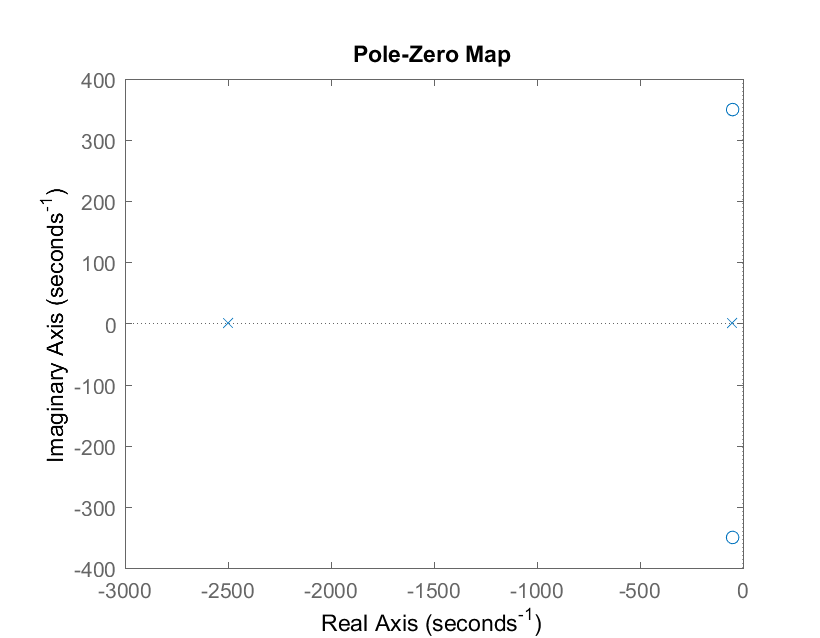
\includegraphics[width=4.51866in,height=3.51574in]{../../Images/PolesAndZeroesQ2.png}

What could its transfer function be? \\

a.\(\text{\ H}\left( s \right) = \frac{s + 350}{s + 1275}\).

b.\(\text{\ H}\left( s \right) = \frac{(s + 50)(s + 2500)}{\left( s + 50 \right)^{2} + 350^{2}}\).

*c.\(\text{\ H}\left( s \right) = \frac{\left( s + 50 \right)^{2} + 350^{2}}{\left( s + 50 \right)\left( s + 2500 \right)}\).

d.\(\text{\ H}\left( s \right) = \frac{\left( s + 50 \right)^{2} - 350^{2}}{\left( s + 50 \right)\left( s + 2500 \right)}\).

e. I do not know. \\
